\documentclass[times, twoside, watermark]{zHenriquesLab-StyleBioRxiv}

% Note: Write each sentence on its own line (makes diffs easier to read).

% Please give the surname of the lead author for the running footer
\leadauthor{Khurana}

\begin{document}

%\title{pykarambola: a Python package for Minkowski tensor analysis of 3D triangulated surfaces}
\title{pykarambola: Minkowski tensor morphometry of 3D biological structures}
\shorttitle{pykarambola}

% Use letters for affiliations, numbers to show equal authorship (if applicable) and to indicate the corresponding author
\author[1]{Yajushi Khurana}
\author[1,\Letter]{Keisuke Ishihara}

\affil[1]{Department of Computational and Systems Biology, School of Medicine, University of Pittsburgh, Pittsburgh, PA, USA}
\maketitle

%TC:break Abstract
\begin{abstract}
% TODO (issue #22): Write abstract
\end{abstract}
%TC:break main

\begin{keywords}
Minkowski tensors | morphometry | 3D image analysis | Python | bioimage analysis
\end{keywords}

\begin{corrauthor}
ishihara\at pitt.edu
\end{corrauthor}


%% -------------------------------------------------------
\section*{Introduction}
%% -------------------------------------------------------

% TODO (issue #23): Minkowski functionals and tensors

% TODO (issue #25): Python ecosystem and bioimage analysis community
Modern bioimage analysis relies on open source tools largely written in Python.
A typical morphometry pipeline proceeds from microscopy acquisition through volumetric segmentation to quantitative shape measurement, with tools such as scikit-image~\cite{vanderwalt2014scikit} for image processing and surface extraction, napari~\cite{Sofroniew2026napari} for interactive 3D visualisation, and pandas~\cite{McKinney2010pandas} for tabular data handling.
Most morphometry tools in this ecosystem report simple scalar descriptors (volume, surface area, sphericity) that do not capture the directional properties of shape.
Approaches based on spherical harmonics~\cite{ruan2019evaluation, viana2023integrated} capture richer structural information but are restricted to genus-zero surfaces and do not generalise to objects with complex 3D topology.
Minkowski tensors capture directional information explicitly: their eigensystems directly quantify elongation and orientation, which are biologically relevant for polarised cells, elongated organelles, and anisotropic tissue architecture.
While computing Minkowski tensors on 3D triangulated surfaces is possible in C++ (karambola~\cite{Schaller2020karambola}), but it is not directly accessible within Python workflows.
Here we present our tool pykarambola, a Python package that integrates Minkowski tensor analysis directly into the Python bioimage ecosystem: in a single call, segmented objects are converted into triangulated surfaces and processed into a dict of NumPy arrays with the objects' corresponding Minkowski tensors, which makes its output immediately compatible with downstream analysis and mesh visualisation tools~\cite{Sofroniew2026napari, Sullivan2019pyvista, Musy2026vedo}.

% TODO (issue #24): karambola C++ and motivation for a Python port
The C++ karambola package~\cite{Schaller2020karambola} is the reference implementation for computing Minkowski tensors on 3D triangulated surfaces, and has been widely used in structural analysis of soft matter and disordered systems~\cite{SchroderTurk2013}.
It accepts meshes in two formats: the karambola-native \texttt{.poly} format and the Object File Format (\texttt{.off}), and writes results to plain-text files.
Despite its numerical capabilities, karambola is not distributed through a package manager, requires a C++ build toolchain, and provides no NumPy-compatible interface.
Researchers who wish to use it within a Python pipeline must write format-conversion scripts for the input and output parsers around the binary, adding fragile intermediates that are difficult to maintain.
pykarambola removes these barriers: it is installable with \texttt{pip install pykarambola}, extends input support to Wavefront OBJ (\texttt{.obj}) and binary glTF (\texttt{.glb}) in addition to \texttt{.poly} and \texttt{.off}, accepts vertex and face arrays directly as NumPy arrays, and returns results as plain Python dicts.



%% -------------------------------------------------------
\section*{Methods}
%% -------------------------------------------------------

\subsection*{Architecture of pykarambola}
pykarambola is a complete Python reimplementation of the C++ karambola package~\cite{Schaller2020karambola}.
The port reproduces the logical structure of the C++ source: a \texttt{Triangulation} class holds the surface mesh and precomputed per-triangle and per-edge geometry, a set of \texttt{calculate\_w*} functions implements the Minkowski tensor formulae, and a command-line interface reproduces the behavior of the original binary.
The C++ implementation depended on the GNU Scientific Library (GSL) for eigenvalue decomposition; pykarambola replaces this with NumPy's \texttt{eigh} routine, removing the only non-Python build dependency from the core computation.

The package is structured around a pure-Python core that requires NumPy~\cite{harris2020numpy} and SciPy~\cite{virtanen2020scipy}.
SciPy is used for connected component detection on mesh graphs and for spherical harmonic basis functions in the spherical Minkowski summary quantities (\texttt{msm}).
An optional Cython extension accelerates the graph-traversal steps of mesh initialisation; the package falls back to pure-Python implementations when the extension is absent (described below).
The API for computing Minkowski tensors directly from segmented 3D label images (\texttt{minkowski\_tensors\_from\_label\_image}) requires scikit-image~\cite{vanderwalt2014scikit} for marching-cubes surface extraction; this dependency is not declared as mandatory and resolves automatically in environments where scikit-image is already present.

Pykarambola retains support for the two mesh formats accepted by C++ karambola: the karambola-native \texttt{.poly} format and the Object File Format (\texttt{.off}).
Two additional parsers for Wavefront OBJ (\texttt{.obj}) and binary glTF (\texttt{.glb}) were added to broaden compatibility with mesh files produced by common 3D reconstruction and visualisation tools.

The Python port and software development were assisted by Claude (Opus 4.5 and Sonnet 4.6; Anthropic).
Numerical correctness of the port was validated by extensive benchmarking against the C++ karambola binary across a diverse set of test meshes, confirming agreement to floating-point precision for all Minkowski scalars, vectors, and tensors.

\subsection*{Acceleration strategy: NumPy vectorization and Cython}
The primary performance strategy in pykarambola is NumPy vectorization~\cite{harris2020numpy}.
Rather than iterating over individual triangles or edges in Python, all mesh data are stored as contiguous NumPy arrays and bulk array operations are applied across the entire mesh at once.
During \texttt{Triangulation} construction, triangle normals, face areas, triangle centroids, edge lengths, and dihedral angles are precomputed in a single vectorized pass using batched cross-products and array-wise norm computations on $(F \times 3)$ arrays, where $F$ is the number of triangles.
Each Minkowski tensor function then reduces these precomputed arrays to per-label scalar, vector, or matrix accumulators using \texttt{numpy.sum} and \texttt{numpy.einsum}, with no Python-level loop over faces.

Two initialisation steps resisted vectorization: building the edge-keyed triangle-adjacency table and constructing the compressed-sparse-row vertex-to-triangle lookup table.
Both require sequential insertion into a hash map indexed by vertex-pair keys, a graph-traversal pattern with data-dependent branching that cannot be expressed as bulk array operations.
These two routines are therefore provided as an optional Cython extension (\texttt{\_accel.pyx}) that uses typed memoryviews and eliminates interpreter overhead on the inner loops.
When the extension is not installed, equivalent pure-Python implementations are used as a fallback.

\subsection*{High-level Python API}
pykarambola exposes two high-level functions that accept NumPy arrays and return plain Python dicts.
The first, \texttt{minkowski\_tensors}, accepts an $(V \times 3)$ vertex array and an $(F \times 3)$ integer face array and returns a dict whose string keys (\texttt{w000}, \texttt{w020}, \texttt{w020\_eigvals}, \ldots) map to NumPy scalars, vectors, or matrices.
The \texttt{compute} argument accepts \texttt{'standard'} (14 base tensors plus eigensystems), \texttt{'all'} (adds higher-order terms \texttt{w103}, \texttt{w104}, the spherical Minkowski summary quantities \texttt{msm}, anisotropy indices, and tensor traces, the latter two being pykarambola-specific extensions not present in C++ karambola), or an explicit list of names for selective computation.
When the \texttt{labels} argument is provided as a per-face integer array, or set to \texttt{'auto'} to detect connected components automatically via SciPy, the function returns a nested dict keyed by label.
The \texttt{center} argument controls the reference point for position-dependent tensors: \texttt{None} uses the array origin, \texttt{'reference\_centroid'} reproduces the C++ karambola \texttt{--reference\_centroid} flag, \texttt{'centroid\_mesh'} shifts each object to its volume-weighted center of mass before computing, and an explicit $(3,)$ array applies a fixed shift; the boolean \texttt{center\_per\_label} (default \texttt{True}) determines whether centroid shifts are computed independently per labeled object or from the whole mesh.
The second, \texttt{minkowski\_tensors\_from\_label\_image}, accepts a three-dimensional integer NumPy array in which each nonzero value identifies an object.
It extracts a triangulated isosurface for each label via \texttt{scikit-image} marching cubes and returns a dict keyed by integer label with the same structure as the mesh API; the \texttt{spacing} argument propagates physical voxel dimensions to all length, area, and volume quantities, and \texttt{autolabel=True} treats the array as a binary mask and delegates connected-component splitting to the mesh API.


%% -------------------------------------------------------
\section*{Results}
%% -------------------------------------------------------

\subsection*{Runtime benchmark}

We benchmarked pykarambola against the reference C++ karambola binary on two mesh sets.
First, synthetic icospheres at subdivision levels 5–10 (10{,}242 to 10{,}485{,}762 vertices) were used to characterise runtime scaling; both the pure-Python build and the Cython-accelerated build were timed independently (see Acceleration strategy, Methods).
Second, the AdrenalMNIST3D a standardized biomedical dataset~\cite{Yang2023MedMNIST} with 1{,}584 adrenal glands at two voxel resolutions (28$^3$ and 64$^3$) was used to measure performance on realistic biological meshes.
All measurements were performed on a single core of an Apple~M4 processor (macOS~15.7.3, Python~3.11).

On icospheres, the Cython-accelerated build reduced compute time by ~1.5–1.9$\times$ relative to the pure-Python build, with the largest gain at smaller mesh sizes where interpreter overhead in the graph-traversal routines is proportionally greater (Figure~\ref{fig:runtime}).
End-to-end (file parse plus compute), pykarambola was 2.0–2.2$\times$ faster than C++ karambola across all mesh sizes; the Cython-accelerated build reached 2.7–3.4$\times$ faster.
On AdrenalMNIST3D, pykarambola processed all 1{,}584 meshes at 28$^3$ resolution in 22~s versus 92~s for C++ karambola (4.1$\times$ faster) and at 64$^3$ resolution in 112~s versus 221~s (2.0$\times$ faster), for a 2.3$\times$ combined speedup.
The C++ karambola timing includes sequential file I/O (one result folder per mesh written to disk), whereas the pykarambola timing covers only in-memory computation; the I/O overhead of the C++ binary partially accounts for the speedup observed on the adrenal dataset.

\begin{figure}
\centering
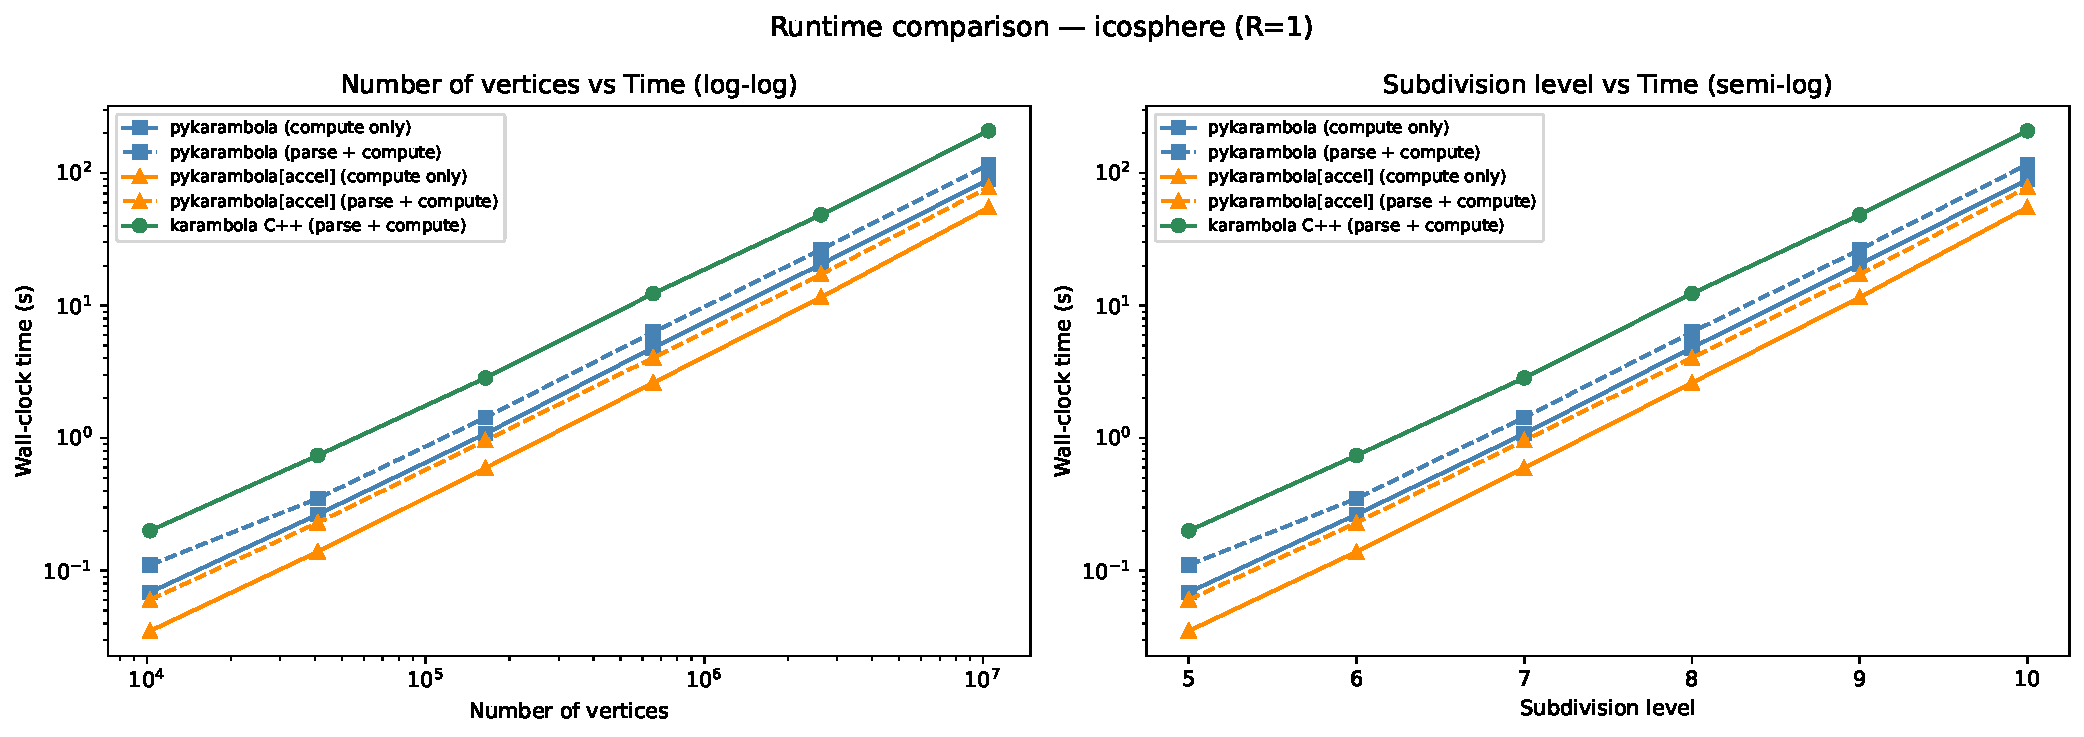
\includegraphics[width=\linewidth]{notebooks/results/timing_comparison.pdf}
\caption{Runtime benchmark comparing pykarambola and C++ karambola as a function of mesh size.}
\label{fig:runtime}
\end{figure}

\subsection*{Numerical accuracy}

We compared pykarambola output to C++ karambola on the full AdrenalMNIST3D dataset~\cite{Yang2023MedMNIST} (1{,}584 meshes at both 28$^3$ and 64$^3$ resolutions), evaluating all scalar, vector, tensor and tensor eigenvalue features returned by the standard computation mode.
In addition, the anisotropy indices for the adrenal meshes were computed.
For 73 of the 76 features, mean relative error was below $3 \times 10^{-5}$\% and maximum relative error was below $3.5 \times 10^{-3}$\% at 28$^3$ resolution and below $0.73$\% at 64$^3$ resolution, confirming agreement at floating-point precision across all Minkowski scalars, vectors, and tensors (Figure~\ref{fig:accuracy}).

Three features showed elevated mean relative errors: the three \texttt{w010} components (the center-of-mass position vector), \texttt{w300} (the integral of mean curvature), and the \texttt{w202\_02} off-diagonal tensor element.
For \texttt{w010}, elevated errors arise because the AdrenalMNIST3D meshes are center-of-mass aligned to the origin, making all three components physically near zero; any small absolute floating-point discrepancy between the two implementations then inflates the relative error.
For \texttt{w300} and \texttt{w202\_02}, a subset of meshes produces values within machine epsilon of zero, again causing the relative error metric to be uninformative.
In all cases, inspection of the highest-error instances confirmed that both implementations return values consistent with physical zero, and their absolute errors are within floating-point precision ($\lesssim 10^{-8}$).
The residual discrepancies observed in non-near-zero features arise from differences in floating-point evaluation order between the C++ and Python implementations and from the substitution of the GNU Scientific Library eigenvalue solver with NumPy's \texttt{eigh}; both sources affect only the last 1--2 significant digits.

\begin{figure}
\centering
% TODO (issue #20): Figure — numerical accuracy agreement with C++ karambola
\caption{Numerical accuracy of pykarambola relative to the reference C++ karambola implementation.}
\label{fig:accuracy}
\end{figure}

\subsection*{Label-image API walkthrough}
% TODO (issue #33)

\begin{figure}
\centering
% TODO (issue #18): Figure — Minkowski tensor computation pipeline schematic
\caption{Schematic of the Minkowski tensor computation pipeline in pykarambola.}
\label{fig:pipeline}
\end{figure}

\begin{figure}
\centering
% TODO (issue #21): Figure — label-image API single-label vs multi-label
\caption{Label-image API applied to a 3D binary image: single-label versus multi-label mode.}
\label{fig:labelimage}
\end{figure}


%% -------------------------------------------------------
\section*{Discussion}
%% -------------------------------------------------------
% TODO (issue #34)


%% -------------------------------------------------------
\section*{Conclusions}
%% -------------------------------------------------------
% TODO (issue #35)


%% -------------------------------------------------------
\section*{Software availability}
%% -------------------------------------------------------
pykarambola is available at \url{https://github.com/Ishihara-SynthMorph/pykarambola}.
Core dependencies are NumPy and SciPy; optional dependencies include Cython (for acceleration) and scikit-image (for label-image API).
% TODO (issue #36): Complete software availability statement


\begin{acknowledgements}
pykarambola is a GPL\,3.0 derivative work of karambola, the C++ reference implementation by Schaller, Kapfer, and Schröder-Turk~\cite{Schaller2020karambola}.
This work was supported in part by an American Heart Association Career Development Award (grant 25CDA1432232) to K.I.
\end{acknowledgements}

\begin{contributions}
Y.K.\ and K.I.\ contributed equally to Software.
Y.K.: Methodology, Validation, Visualization, Writing -- original draft.
K.I.: Conceptualization, Funding acquisition, Project administration, Supervision, Writing -- review \& editing.
\end{contributions}

\section*{Bibliography}
\bibliography{references}

%TC:ignore
\onecolumn
\newpage

\section*{Word Counts}
\subsection*{Statistics on word count}
\detailtexcount

%TC:endignore

\end{document}
